\chapter[Resultados, Mediciones y Verificación]{Resultados, mediciones y verificación} \label{sec:resultados}

\section{Resultados del acoplador híbrido en cuadratura} \label{sec:resultados_acoplador}
El acoplador híbrido en cuadratura fue caracterizado experimentalmente en sus dos versiones fabricadas, midiendo los prototipos tanto en CNEA (Figura~\ref{fig:coupler_cnea_setup}) como en UTN, de acuerdo con la metodología descripta en la Sección~\ref{sec:metodologia_medicion}. A continuación se presentan dichos resultados, junto con la comparación frente a los obtenidos mediante simulación en ADS y en CST.

\begin{figure}[H]
    \centering
    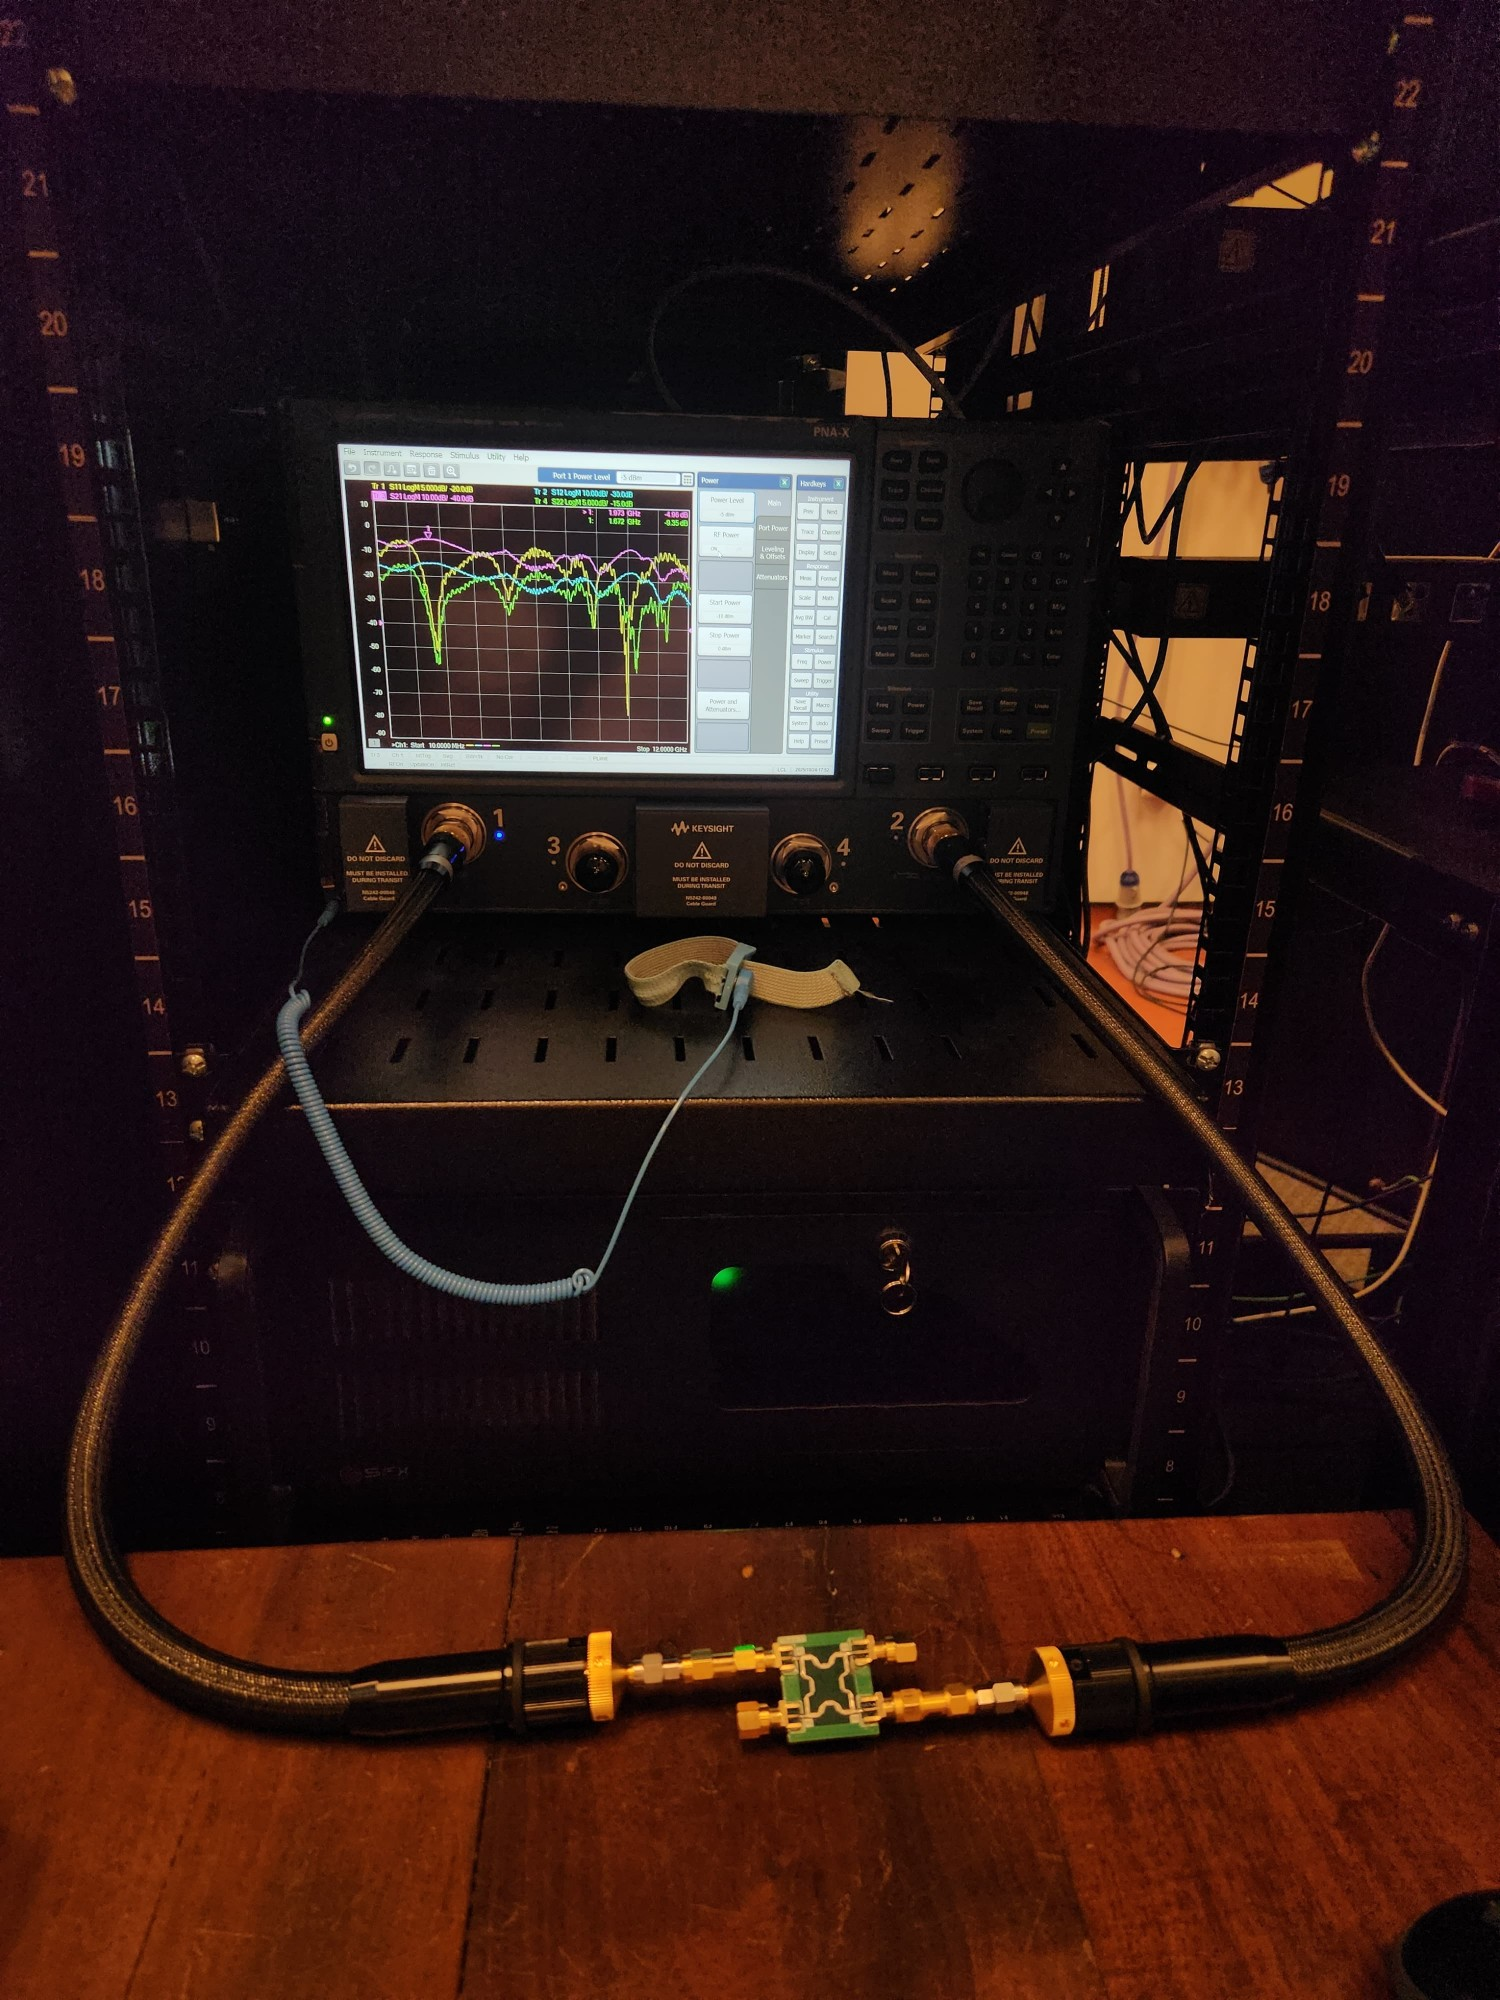
\includegraphics[width=0.55\linewidth]{Figures/08/coupler_cnea_setup.png}
    \caption{Medición del acoplador con el VNA N5242B PNA-X en CNEA.}
    \label{fig:coupler_cnea_setup}
\end{figure}

\subsection{Comparación entre versiones del acoplador}
La Figura~\ref{fig:coupler_reflexion_v1_v2} muestra los parámetros de reflexión medidos en los puertos 1, 2 y 3 para ambas versiones del acoplador, donde se observa claramente el corrimiento de la frecuencia de adaptación entre ambas versiones, corroborando las simulaciones que se llevaron a cabo.

\begin{figure}[H]
    \centering
    \begin{subfigure}{0.48\linewidth}
        \centering
        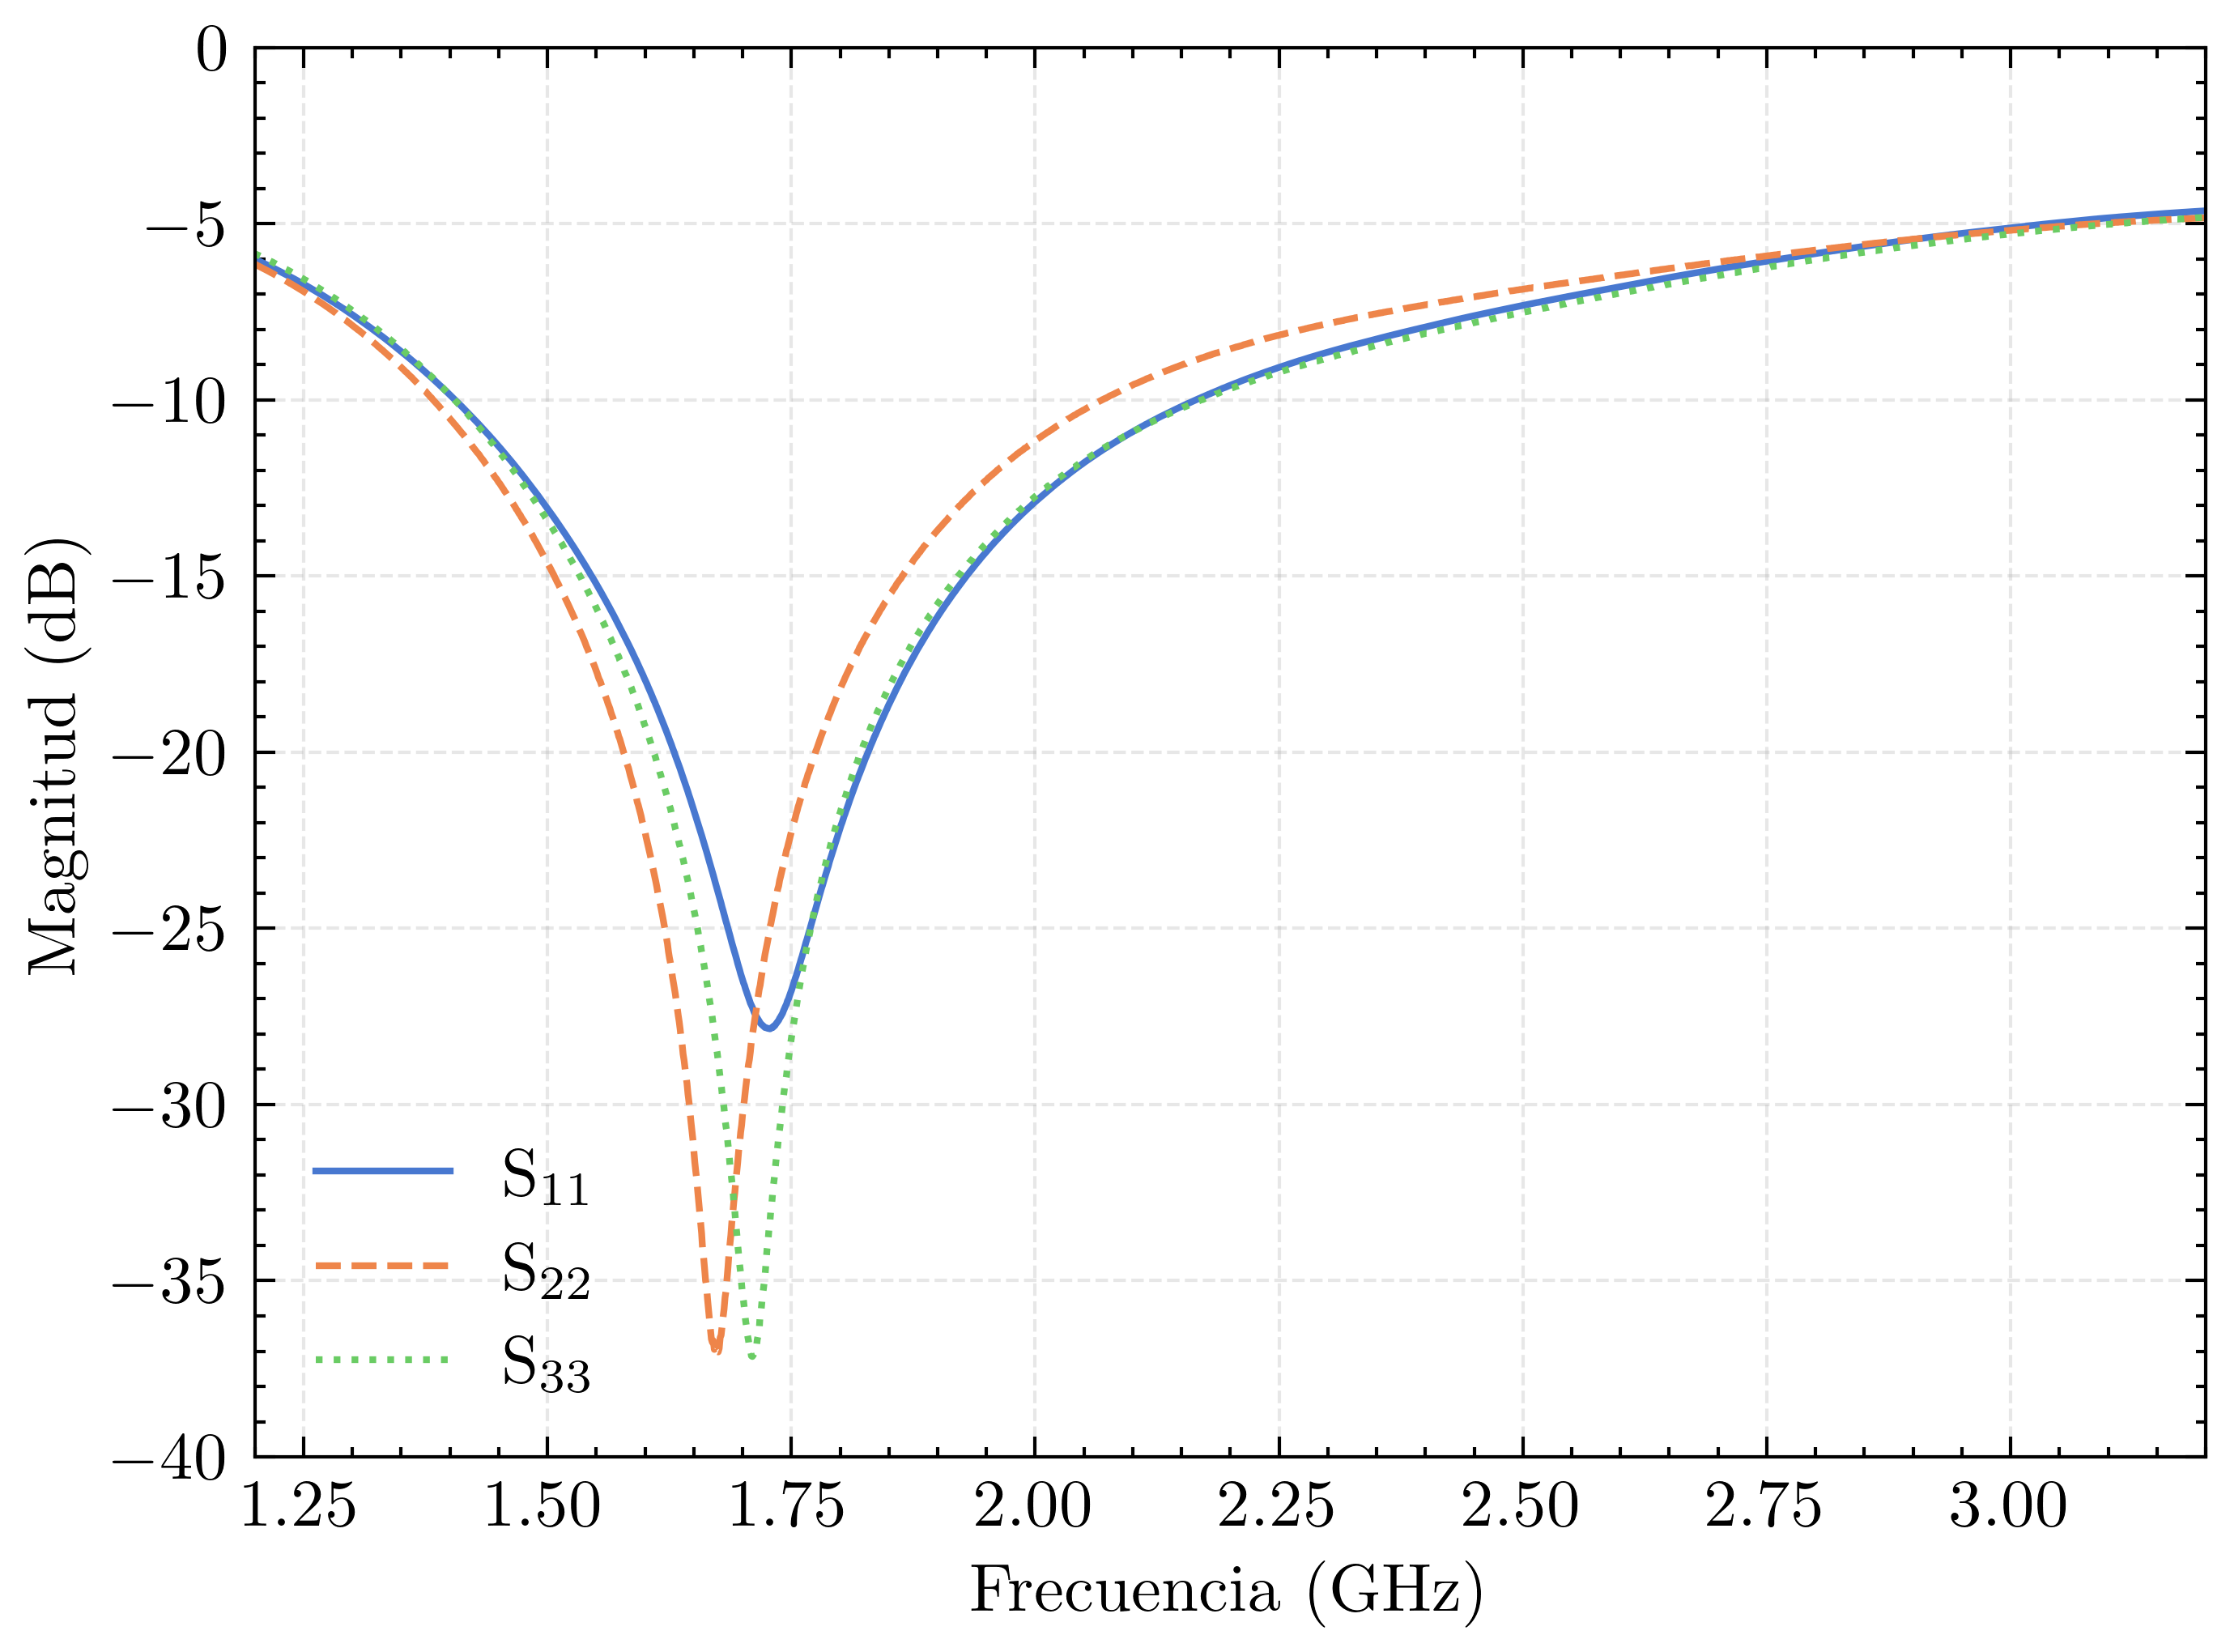
\includegraphics[width=\linewidth]{Figures/08/coupler_reflexion_v1.png}
    \end{subfigure}
    \hfill
    \begin{subfigure}{0.48\linewidth}
        \centering
        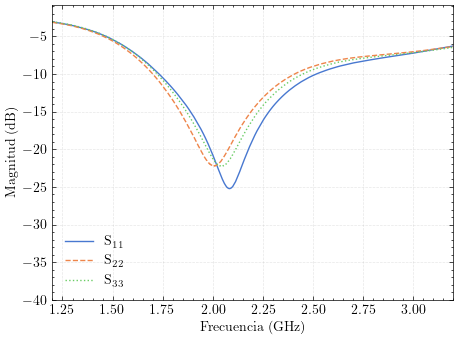
\includegraphics[width=\linewidth]{Figures/08/coupler_reflexion_v2.png}
    \end{subfigure}
    \caption{Parámetros de reflexión medidos en los puertos 1, 2 y 3 del acoplador. Izquierda: primera versión. Derecha: segunda versión.}
    \label{fig:coupler_reflexion_v1_v2}
\end{figure}

De la Figura~\ref{fig:coupler_reflexion_v1_v2} también cabe destacar que la magnitud de $S_{11}$ resulta similar entre ambas versiones. En cambio, los parámetros $S_{22}$ y $S_{33}$ son considerablemente mejores en la primera versión que en la segunda. Si bien el corrimiento de la frecuencia central entre versiones se explica por la incorporación del tramo de línea que modela el pad de conexión del SMA, tal como se detalla más adelante, la diferencia entre las magnitudes de reflexión alcanzadas por cada versión no cuenta con una explicación igualmente clara, y, aunque podría deberse al mismo motivo, también podría deberse a variaciones introducidas durante el proceso de fabricación o ensamblado de cada placa. Asimismo, la variación entre los parámetros de reflexión dentro de una misma versión indica que el acoplador fabricado no se comporta simétricamente, tal como sí lo hace idealmente según la matriz de dispersión de la ecuación~\eqref{eq:quadrature_scattering}, aspecto que debería estudiarse con mayor profundidad en un trabajo futuro.

Por otro lado, para cuantificar la comparación entre versiones en términos de los parámetros de transmisión, el Cuadro~\ref{tab:coupler_v1_v2} resume los valores de frecuencia central efectiva y magnitud de $S_{21}$ y $S_{31}$, junto con la diferencia de fase entre los puertos de salida a 2,2\,GHz, obtenidos para cada versión.

\begin{table}[H]
    \centering
    \caption{Comparación de los parámetros de transmisión medidos entre el acoplador v1 y v2.}
    \label{tab:coupler_v1_v2}
    \begin{tabular}{lcc}
        \hline\hline
        \textbf{Parámetro} & \textbf{Primera Versión} & \textbf{Segunda Versión} \\
        \hline
        Frecuencia central $S_{21}$                           & 1,701~GHz      & 2,019~GHz       \\
        Magnitud $S_{21}$ a 2,2~GHz                  & $-3,52$~dB     & $-3,62$~dB       \\
        Frecuencia central $S_{31}$                           & 1,542~GHz      & 2,117~GHz       \\
        Magnitud $S_{31}$ a 2,2~GHz                  & $-4,14$~dB     & $-4,14$~dB      \\
        Dif. fase ($\phi_{21}-\phi_{31}$) a 2,2~GHz  & $108,73^\circ$ & $92,57^\circ$   \\
        \hline\hline
    \end{tabular}
\end{table}

Si bien las magnitudes de los parámetros de transmisión resultan similares entre ambas versiones, la diferencia de fase de la versión 2 a la frecuencia de interés resulta más próxima al valor ideal de $90^\circ$ que la de la versión 1 ($92,57^\circ$ frente a $108,73^\circ$), cuya diferencia respecto del valor objetivo supera los $10^\circ$, lo cual puede ocasionar efectos distorsivos indeseados en la implementación de un amplificador Doherty. Estos resultados confirman que la incorporación del tramo de línea que modela el pad de conexión del SMA fue la corrección de diseño determinante para acercar el prototipo fabricado tanto a su frecuencia central como a su comportamiento de fase ideales.

\subsection{Comparación entre laboratorios}
Con el objetivo de evaluar la consistencia y repetibilidad de las mediciones, se compararon los resultados de parámetros de transmisión de la versión 2 obtenidos en la UTN (medición preliminar, con el VNA FieldFox) contra los obtenidos en CNEA (medición definitiva, con el PNA-X), presentados en la Figura~\ref{fig:coupler_utn_vs_cnea}.

\begin{figure}[H]
    \centering
    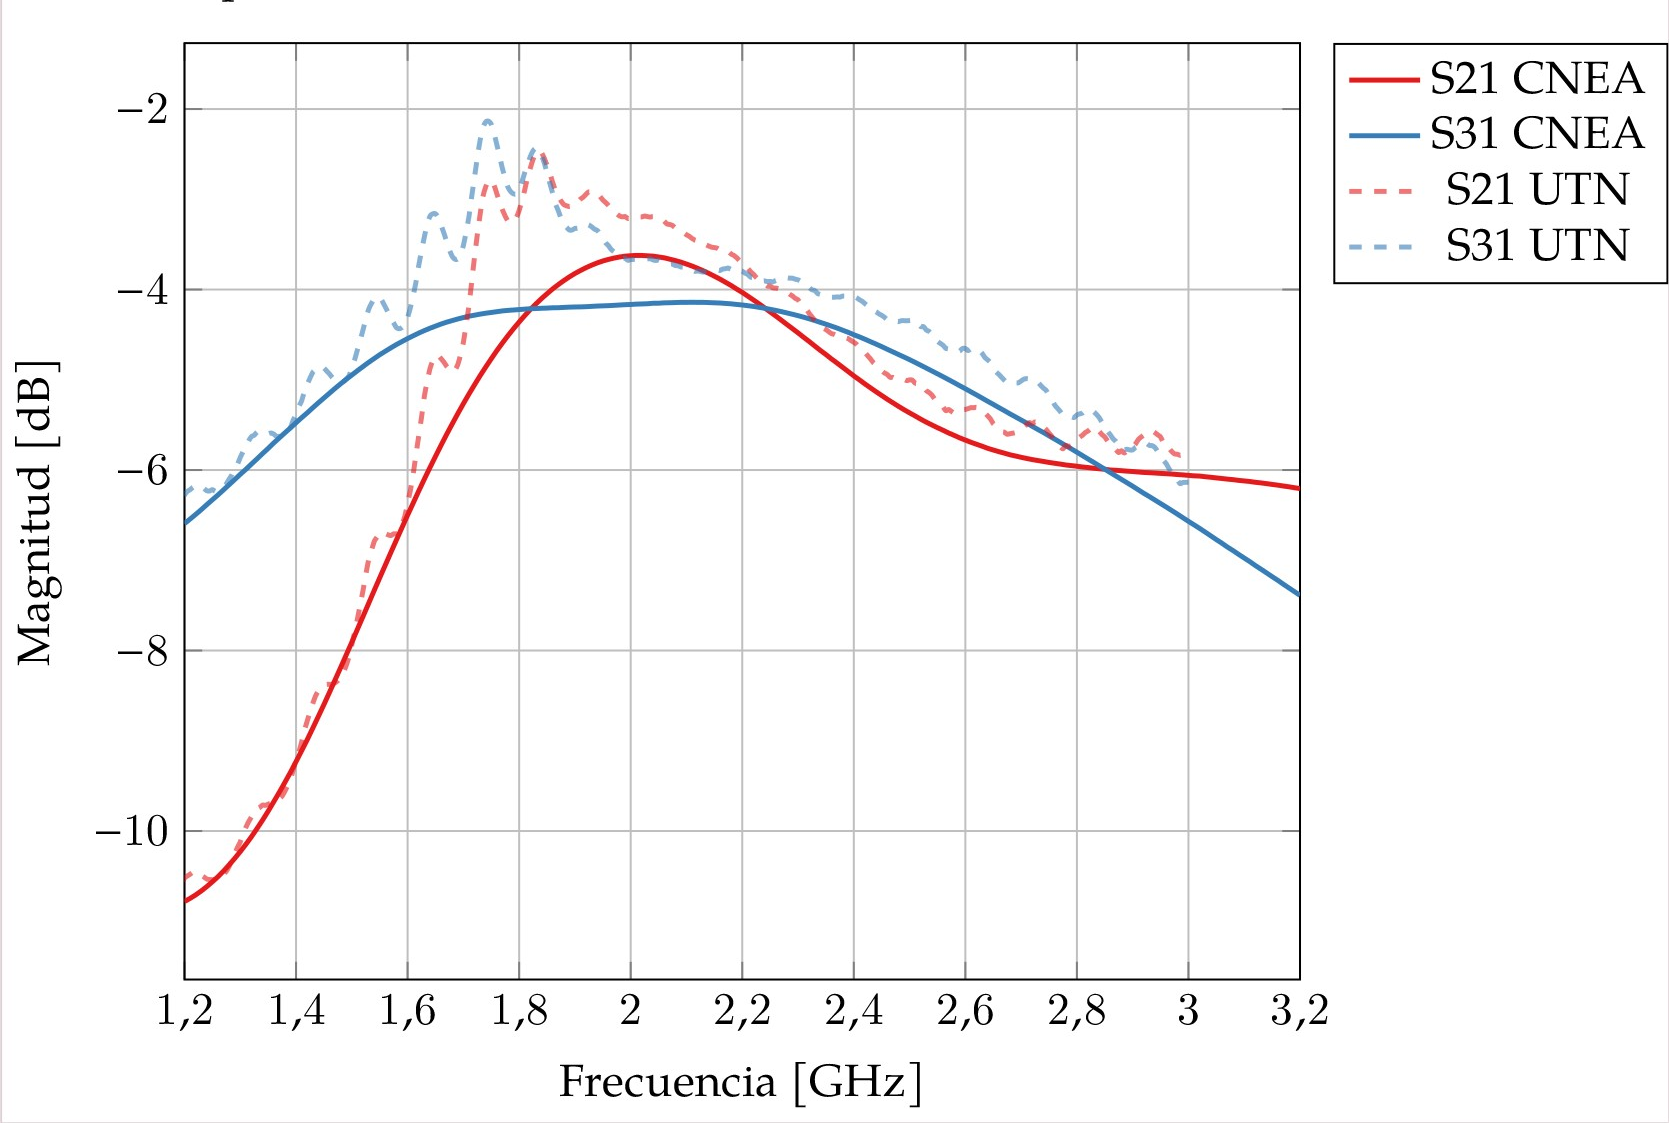
\includegraphics[width=0.85\linewidth]{Figures/08/coupler_utn_vs_cnea.png}
    \caption{Comparación de los parámetros de transmisión del acoplador v2 medidos en UTN y en CNEA.}
    \label{fig:coupler_utn_vs_cnea}
\end{figure}

Ambos conjuntos de datos presentan una forma general similar, aunque la medición realizada en UTN exhibe un ripple considerable que no está presente en la medición de CNEA. Este ripple se atribuye a tres posibles causas. En primer lugar, a una manipulación poco cuidadosa de los cables durante la medición, dado que las numerosas conexiones y desconexiones realizadas para medir en los distintos puertos implicaron correr y doblar los cables, apartándolos de la posición en la que se realizó la calibración. En segundo lugar, a un posible inconveniente durante el proceso de calibración del instrumento, dado que en una de las calibraciones intentadas el equipo se bloqueó y debió reiniciarse, lo que podría indicar que no estaba operando en condiciones óptimas. Por último, el kit de calibración disponible era para cables tipo N, mientras que para la medición se utilizaron cables SMA. La falta de un kit de calibración apropiado, casi con total seguridad, actuó como fuente de errores añadidos, resultando en la degradación de la calidad de medición.

\subsection{Comparación entre mediciones y simulaciones}
Finalmente, se llevó a cabo la comparación entre los resultados medidos sobre el segundo prototipo fabricado contra los resultados de las simulaciones. La Figura~\ref{fig:coupler_fase_comp} compara la diferencia de fase entre los puertos de salida, mientras que las Figuras~\ref{fig:coupler_s21_comp} y~\ref{fig:coupler_s31_comp} comparan los módulos de $S_{21}$ y $S_{31}$ respectivamente.

\begin{figure}[H]
    \centering
    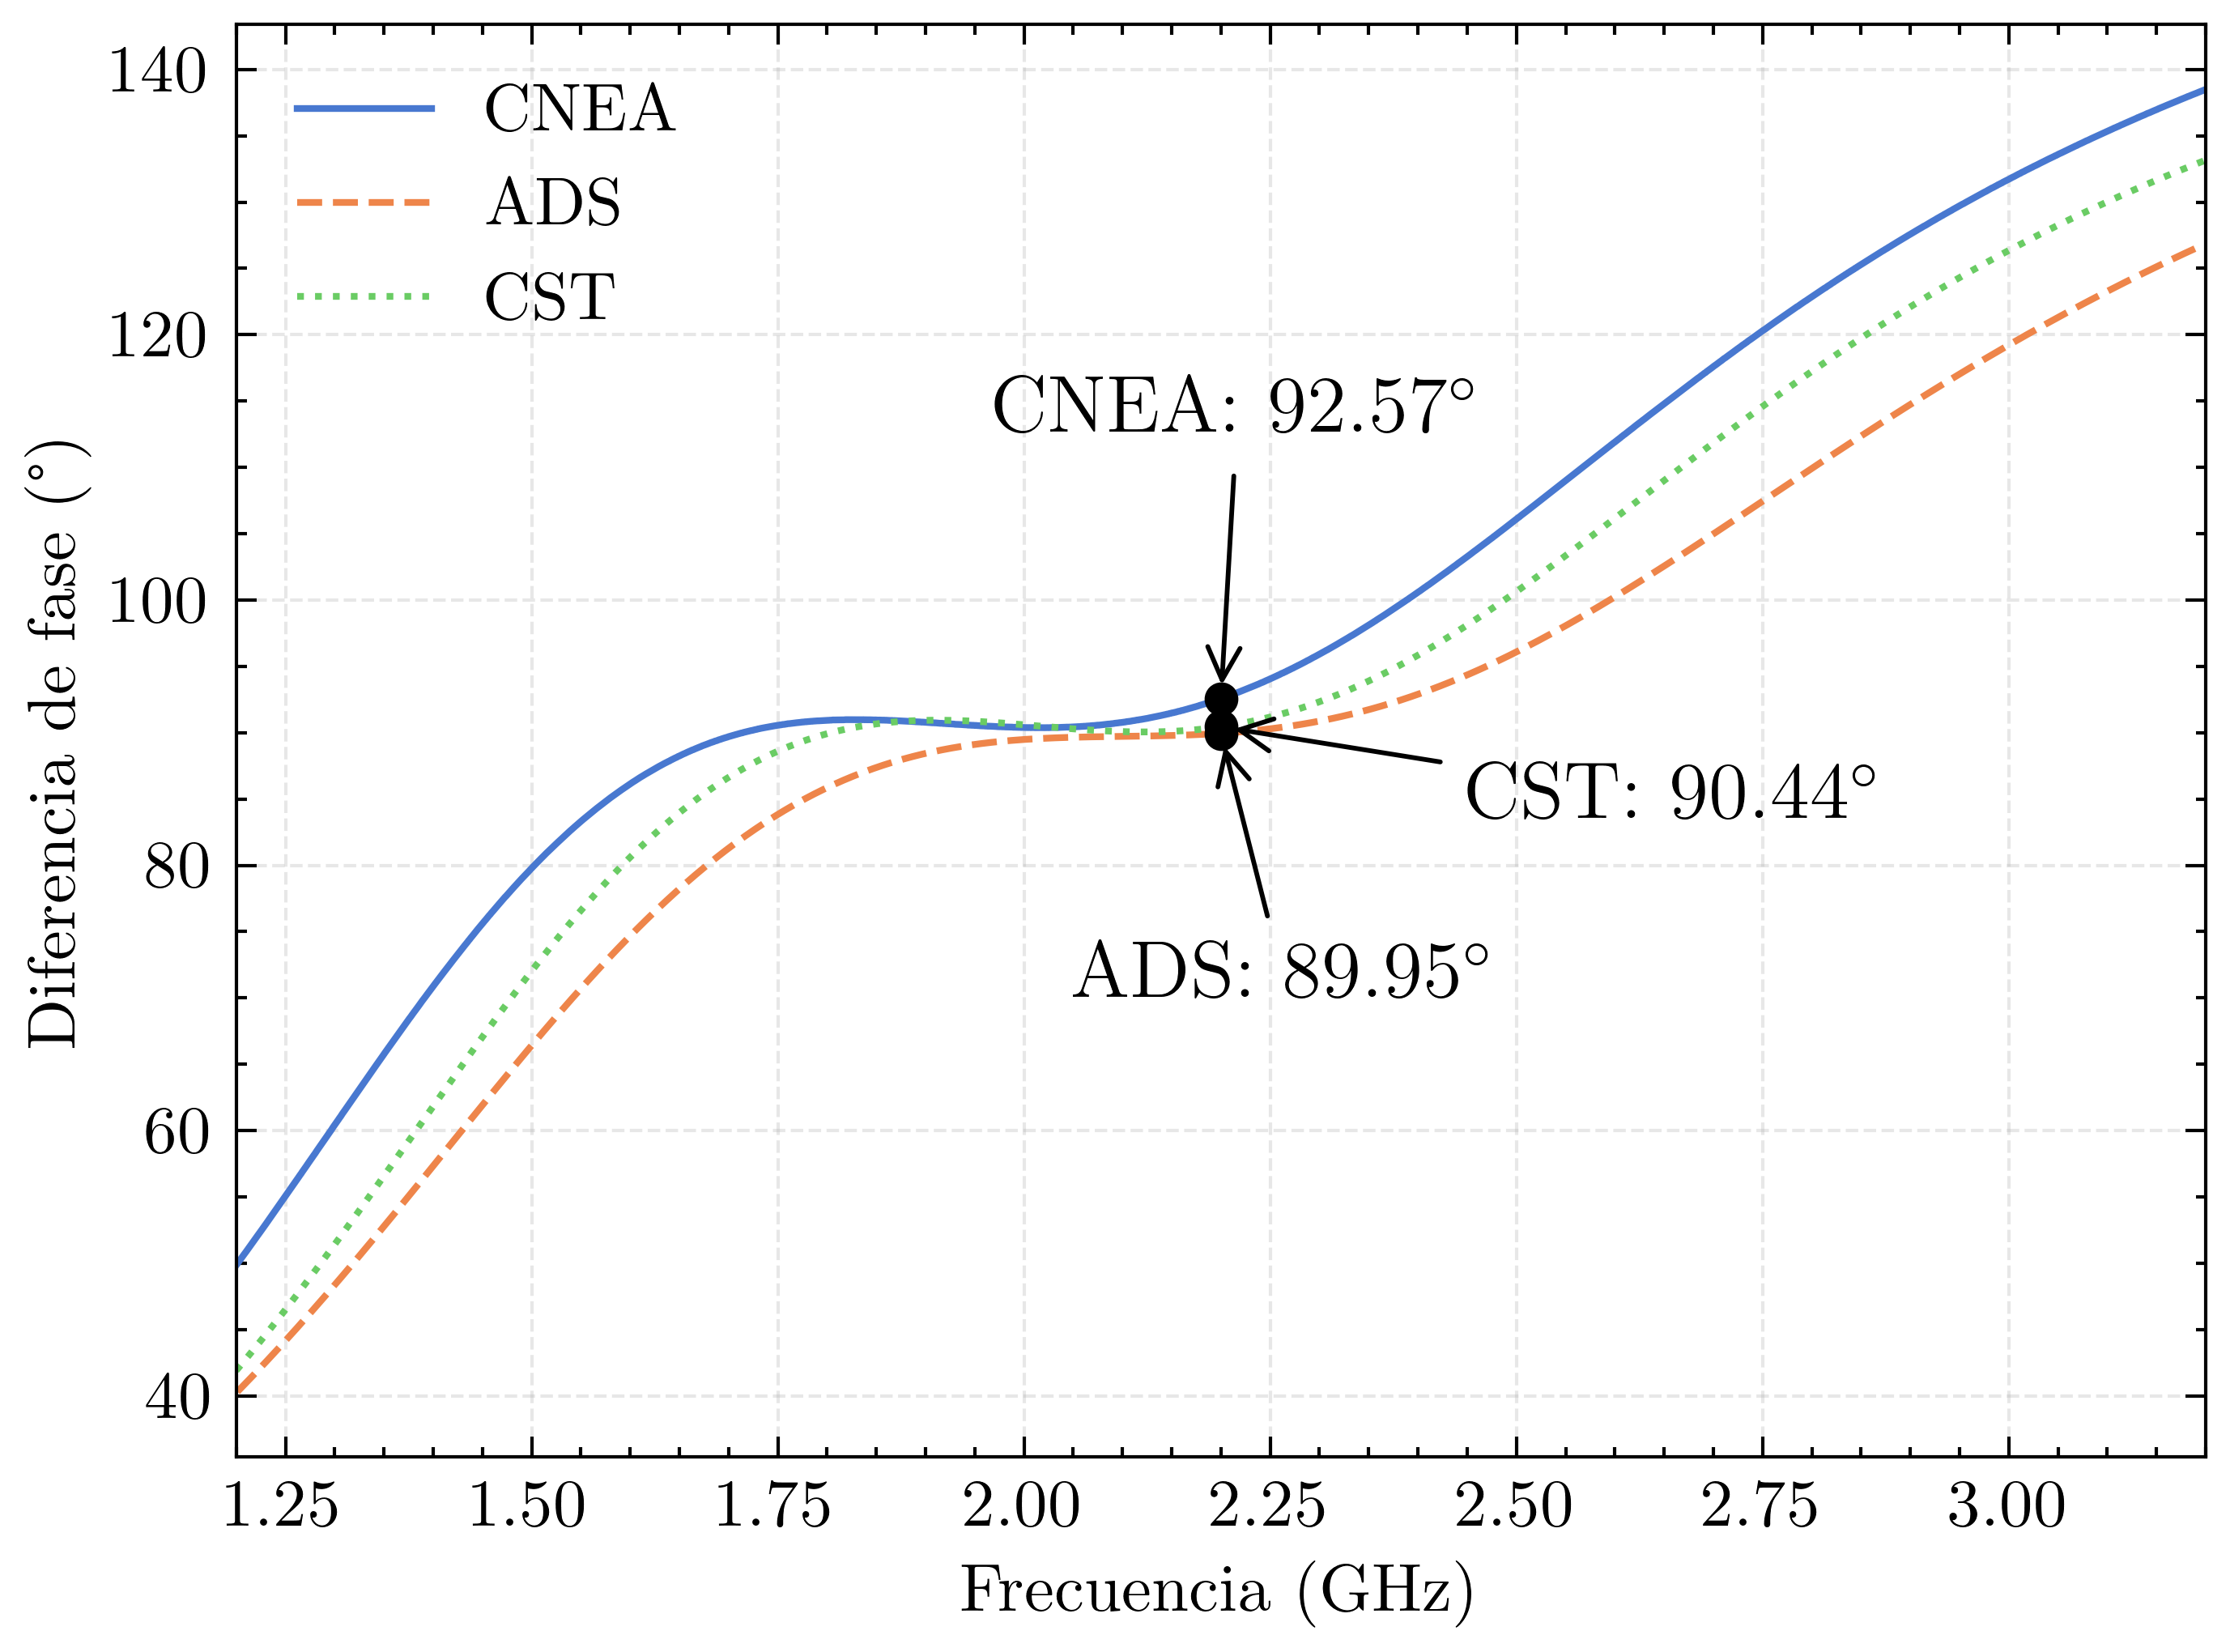
\includegraphics[width=0.85\linewidth]{Figures/08/coupler_fase_lab_ads_cst.png}
    \caption{Comparación de la diferencia de fase entre los puertos de salida medida en laboratorio y simulada en ADS y CST.}
    \label{fig:coupler_fase_comp}
\end{figure}

\begin{figure}[H]
    \centering
    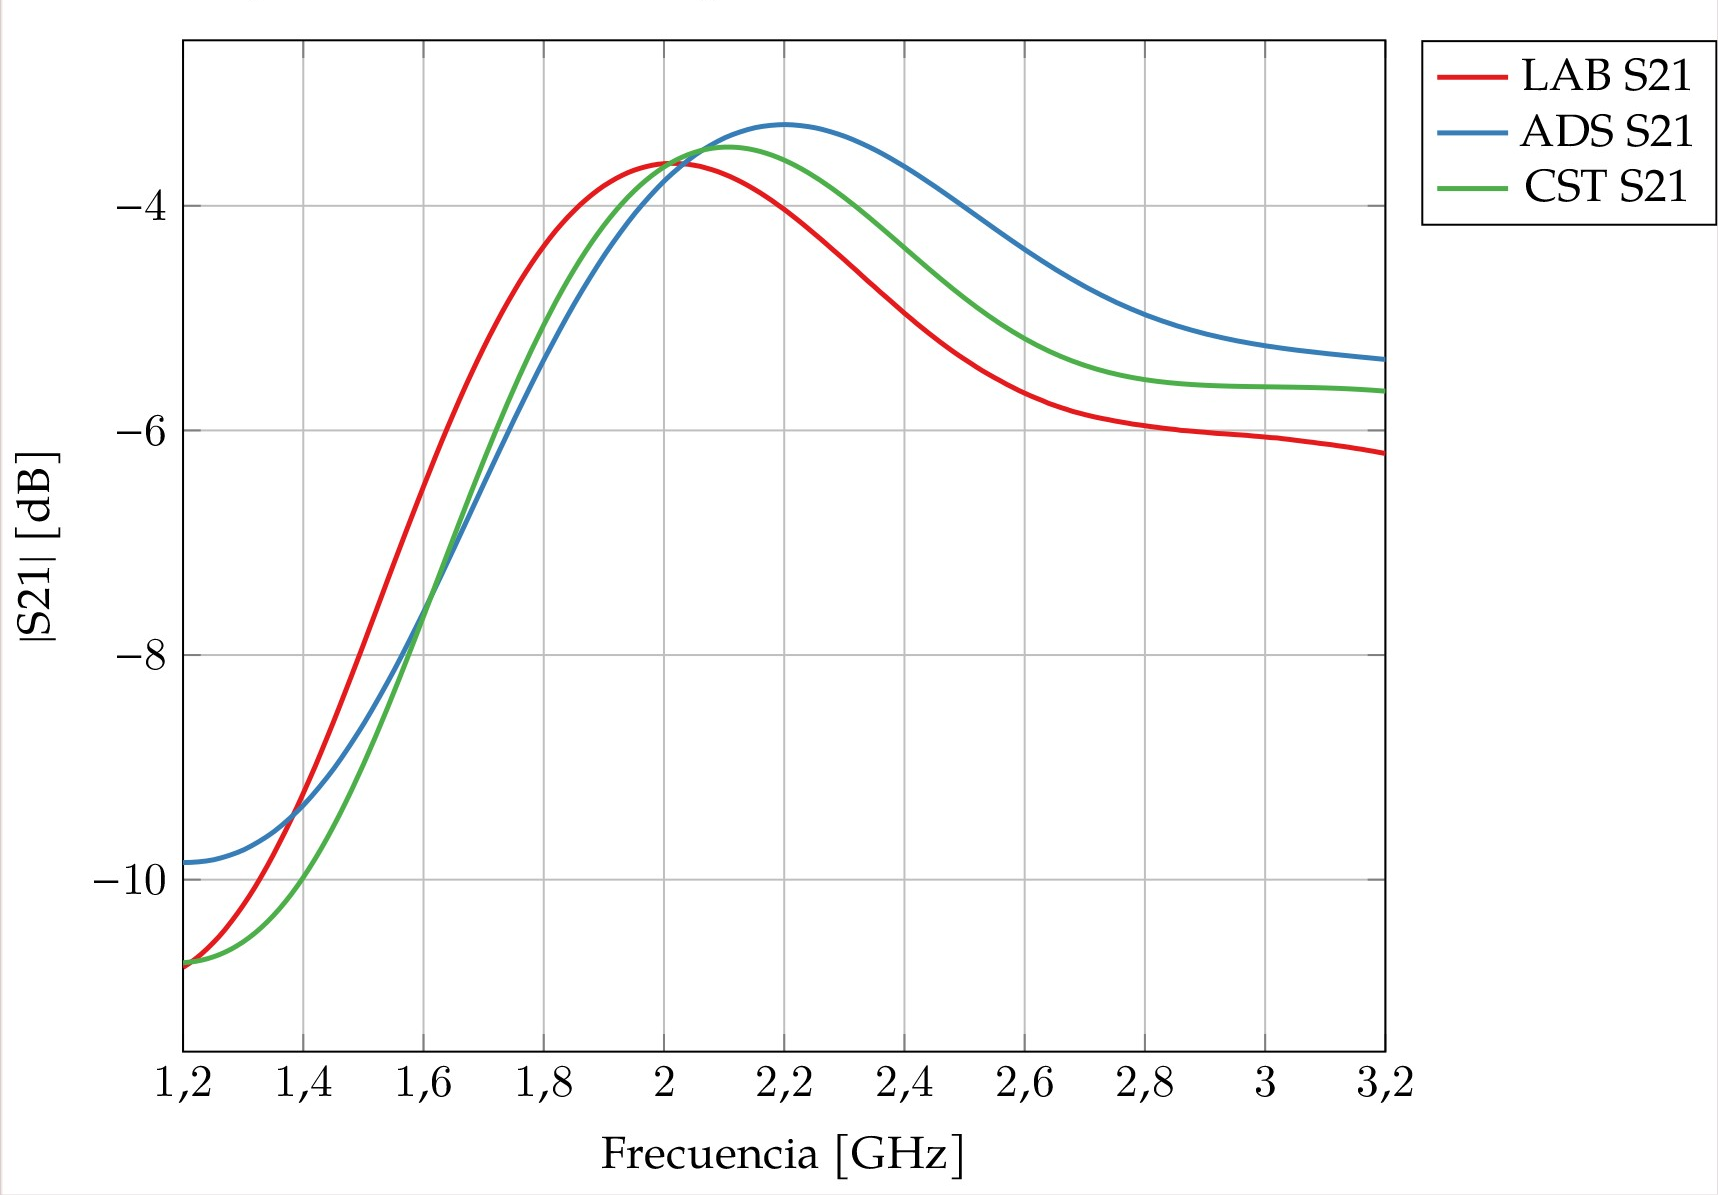
\includegraphics[width=0.85\linewidth]{Figures/08/coupler_s21_lab_ads_cst.png}
    \caption{Comparación del módulo de $S_{21}$ medido en laboratorio y simulado en ADS y CST.}
    \label{fig:coupler_s21_comp}
\end{figure}

\begin{figure}[H]
    \centering
    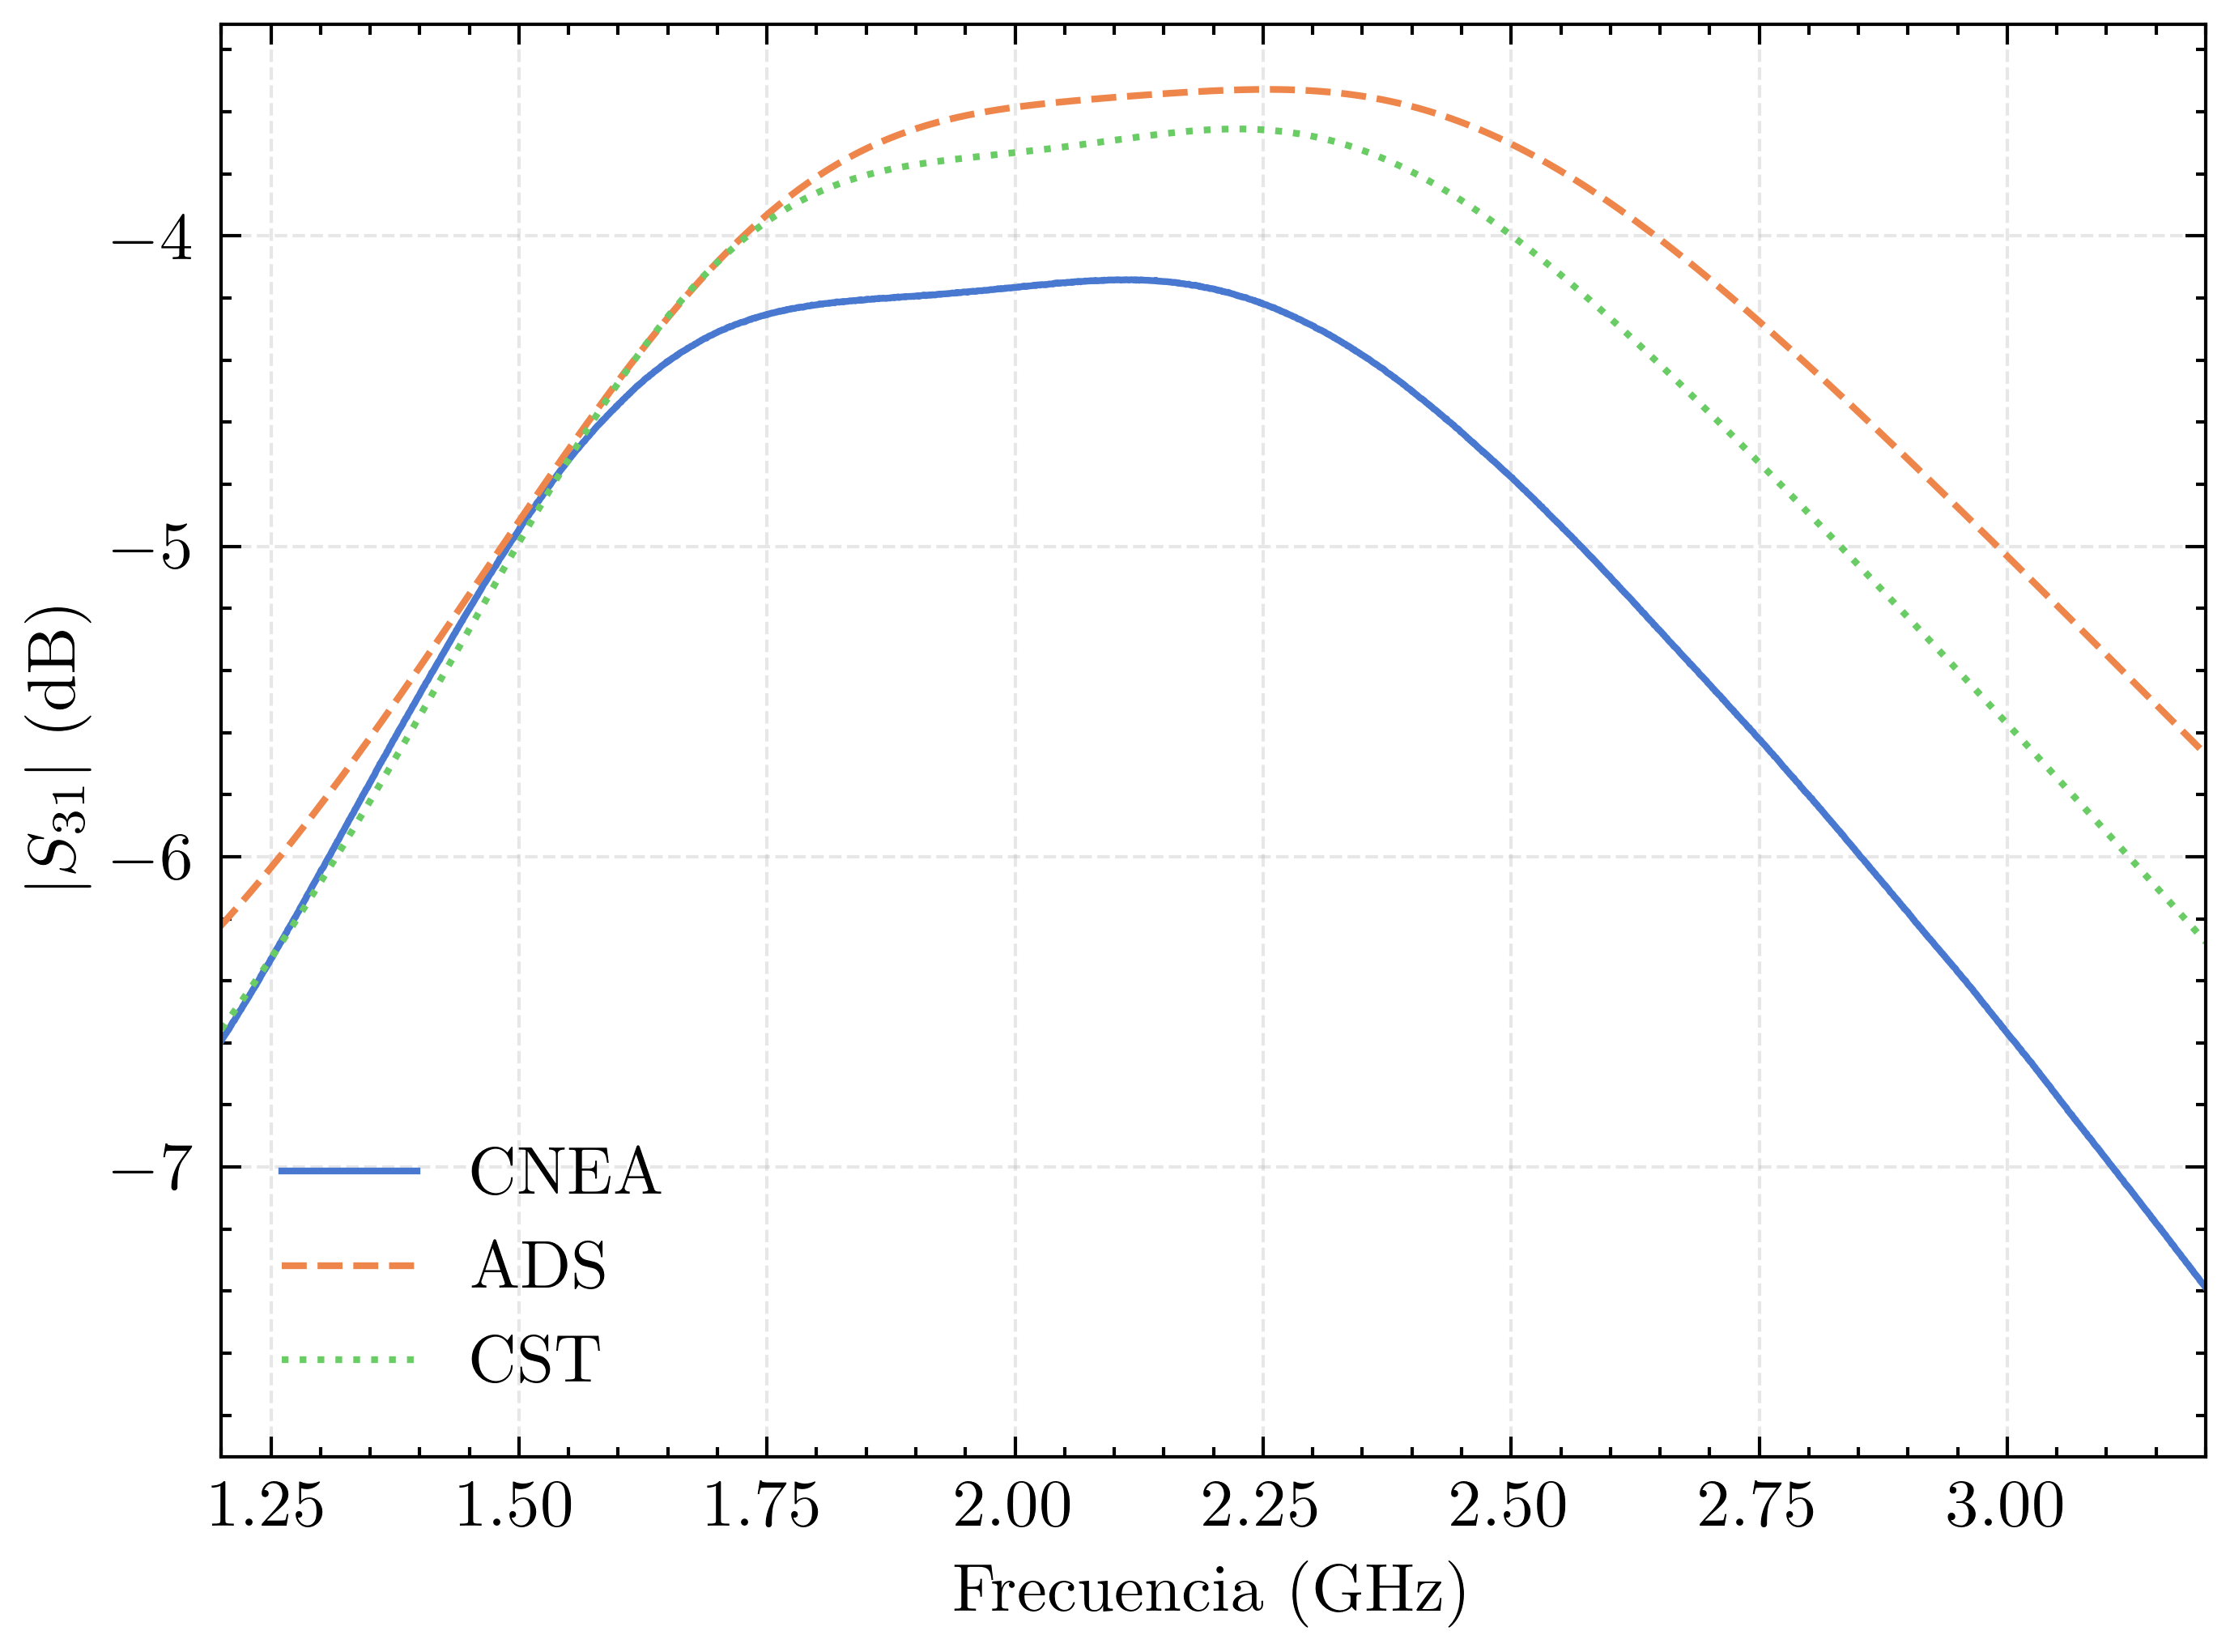
\includegraphics[width=0.85\linewidth]{Figures/08/coupler_s31_lab_ads_cst.png}
    \caption{Comparación del módulo de $S_{31}$ medido en laboratorio y simulado en ADS y CST.}
    \label{fig:coupler_s31_comp}
\end{figure}

El Cuadro~\ref{tab:coupler_lab_ads_cst} resume la comparación de la magnitud de los parámetros de transmisión y la diferencia de fase obtenida en cada caso a la frecuencia de interés de 2,2\,GHz.

\begin{table}[H]
    \centering
    \caption{Diferencia de los parámetros medidos a 2,2\,GHz, medidos y simulados.}
    \label{tab:coupler_lab_ads_cst}
    \begin{tabular}{lccc}
        \hline\hline
        \textbf{Origen} & $\mathbf{|S_{21}|}$ \textbf{(dB)} & $\mathbf{|S_{31}|}$ \textbf{(dB)} & \textbf{Dif. fase} $\mathbf{(\phi_{21}-\phi_{31}) (^\circ)}$ \\
        
        \hline
        Medición (CNEA) & -4,032  & -4,171  & $92,57^\circ$ \\
        Simulación ADS  & -3,227  & -3,3532 & $89,95^\circ$ \\
        Simulación CST  & -3,992  & -3,419  & $90,44^\circ$ \\
        \hline\hline
    \end{tabular}
\end{table}

Los tres resultados de la diferencia de fase se encuentran razonablemente próximos entre sí y al valor ideal de $90^\circ$, siendo la simulación en CST la que mejor se aproxima al valor medido. En cuanto a los módulos de $S_{21}$ y $S_{31}$, la curva medida en laboratorio se encuentra corrida levemente hacia frecuencias más bajas respecto de las curvas simuladas, mientras que las simulaciones en ADS y en CST resultan más próximas entre sí que respecto de la medición.

Del Cuadro~\ref{tab:coupler_lab_ads_cst} se desprende que, tanto en fase como en módulo de los parámetros de transmisión, la simulación electromagnética en CST es consistentemente más cercana a los valores medidos que la simulación esquemática en ADS. La diferencia de fase simulada en CST difiere del valor medido en apenas $2,13^\circ$, frente a los $2,62^\circ$ de diferencia que presenta ADS, y los módulos de $S_{21}$ y $S_{31}$ simulados en CST resultan más próximos a los medidos que los obtenidos en ADS. Esta mayor precisión resulta razonable, dado que CST modela el layout físico completo mediante simulación electromagnética de onda completa, mientras que ADS trabaja sobre un modelo esquemático de líneas de transmisión que no captura en la misma medida los efectos parásitos de la geometría real (discontinuidades y acoplamientos, entre otros). En vista de esto, para un futuro diseño de este mismo circuito podría evaluarse prescindir de la verificación en ADS y emplear directamente CST como única herramienta, tanto para diseño como para simulación electromagnética, ahorrando el paso intermedio sin una pérdida significativa de precisión respecto del comportamiento real del prototipo.
 
Los resultados obtenidos resultan satisfactorios, pero dejan marcado que aún es posible realizar mejoras sobre el diseño. Un cambio de sustrato dieléctrico permitiría reducir aún más las dimensiones del acoplador, dado que la longitud de onda guiada en una línea microstrip es inversamente proporcional a la raíz de la permitividad efectiva del sustrato, un dieléctrico de mayor $\varepsilon_r$ que el FR4 empleado reduciría la longitud física necesaria para cada tramo de $\lambda/4$. Esta reducción, sin embargo, no está exenta de compromisos. Por un lado, para una impedancia característica dada, un sustrato de mayor $\varepsilon_r$ requiere líneas más angostas, lo que incrementa la resistencia serie por unidad de longitud y, en consecuencia, las pérdidas óhmicas del conductor, mientras que las pérdidas dieléctricas dependen de manera independiente de la tangente de pérdidas propia del material elegido. Por otro lado, si bien un mayor $\varepsilon_r$ no afecta directamente al acople de masa en sí, sí endurece indirectamente el criterio de diseño del plano de masa: dado que el criterio de separación entre vías de masa se estableció en términos de una fracción de la longitud de onda guiada ($\lambda/10$), una longitud de onda guiada más corta exige un mallado de vías más denso para mantener la misma continuidad eléctrica del plano de referencia.
 
Finalmente, una mejora adicional sobre el modelo electromagnético empleado consistiría en incorporar en la simulación un modelo tridimensional del conector SMA real, en lugar de la línea de transmisión rectangular con las dimensiones del footprint del pad empleada en este trabajo. Dado que fue precisamente la transición hacia el conector SMA la que introdujo el corrimiento de frecuencia identificado entre el primer y el segundo diseño, un modelo más detallado de dicha transición probablemente reduciría aún más la discrepancia remanente entre los resultados simulados y los medidos.